\paragraph{Цель работы}
Познакомиться с библиотекой React

\paragraph{Задание}
Создать систему авторизации и регистрации пользователя.

В работе использован React, Redux, React-Forms, Redux-Thunk.

\lstinputlisting[language=C++]{../../src/Titles-and-directors/react-front/src/components/login/Login.js}
\lstinputlisting[language=C++]{../../src/Titles-and-directors/react-front/src/components/login/LoginForm.js}
\lstinputlisting[language=C++]{../../src/Titles-and-directors/react-front/src/api/login.js}
\lstinputlisting[language=C++]{../../src/Titles-and-directors/react-front/src/redux/reducers/login-reducer.js}

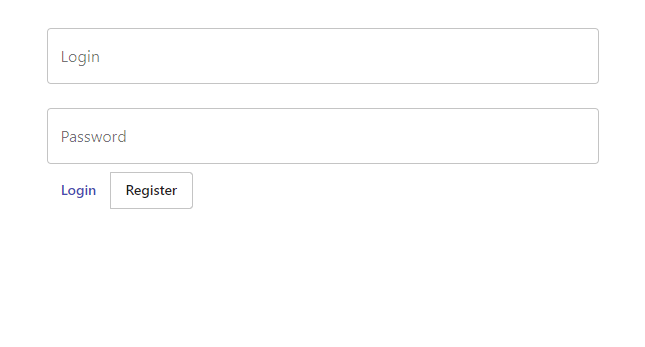
\includegraphics[width=0.6\textwidth]{scr1.PNG}

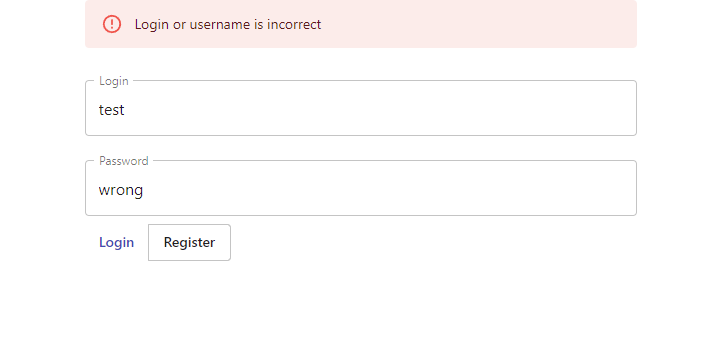
\includegraphics[width=0.6\textwidth]{scr2.PNG}

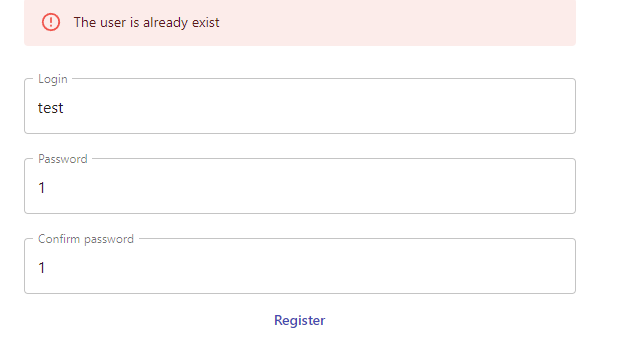
\includegraphics[width=0.6\textwidth]{scr3.PNG}


\includegraphics[width=0.6\textwidth]{scr4.PNG}
